\chapter{Basic Analysis \& Corrections}

\section{Introduction}
This chapter discusses analysis procedures that are common to the subsequent data analyses of kaons.  These procedures can be divided into two groups.  The first type of basic analysis described is the aggregation or calculation of scalar values over the run-period (examples include luminosity and helicity).  The second type of analysis procedure described is a correction to measured values.  Vertex corrections, timing corrections, and kinematic corrections will be discussed.

\section{E1-F}
This study uses the dataset collected between April and July of 2003 known as E1-F.  During this run period the beam energy was 5.498 GeV and the target was a 5cm liquid hydrogen cell.  The torus current was set to 2250 Amperes, to maximize pion acceptance.

\section{Determination of Good Run List}
The total dataset contains 831 runs.  Due to the complexities of the CLAS experimental setup, it is not uncommon for run conditions to change between runs such that a portion of the data collected are not of analysis quality.  For this reason, a good run list is constructed. \\

Good runs are selected for the list by counting good electrons in each file and normalizing by the accumulated charge for the associated file.  For each file, the difference between subsequent Faraday cup readings is summed to calculate the charge for the file.  Creation of the total charge for the run includes an additional contribution from endpoints in adjacent files.  This extra charge builds up after the last scalar reading of one file and before the first scalar bank in the new adjacent file.  While the number of events collected varies from run to run the ratio defined above is a stable quantity -- provided that the run conditions do not vary greatly.  Good runs were chosen to have $N/Q > 4000$ based on inspection of the figure \ref{fig:inclusive_rates}.  The good run list used for this analysis contains 522 runs.  

\begin{figure}
	\label{fig:inclusive_rates}
	\begin{center}
		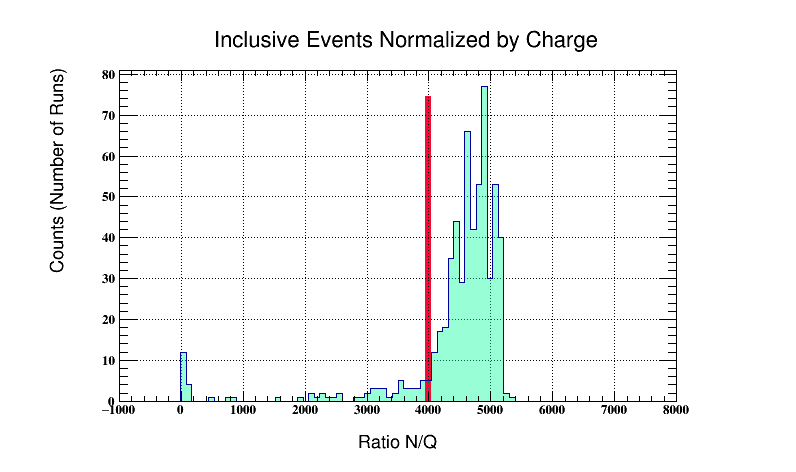
\includegraphics[width=14cm]{image/plots/basic-analysis/inclusive-rates.png}
		\caption{Inclusive electrons per file normalized by the total charge accumulated for the file.  This quantity is used to make a good run list.}
	\end{center}
\end{figure}

\section{Helicity Determination}
During the course of the E1-F run period the beam helicity convention was changed by the insertion of a half-wave plate at the injector.  The definition of $\pm$ helicity must change in accordance with these wave-plate insertions.  To monitor these changes, the value of $A_{LU}^{\sin\phi}$ for $\pi^+$ is recorded for every run.  Whenever the asymmetry (which has a magnitude of around $3\%$) changes sign, the sign convention has changed (see figure \ref{fig:bsa_waveplate}.  These changes are taken into account in the data analysis.   

\begin{figure}
	\centering
	\label{fig:bsa_waveplate}
	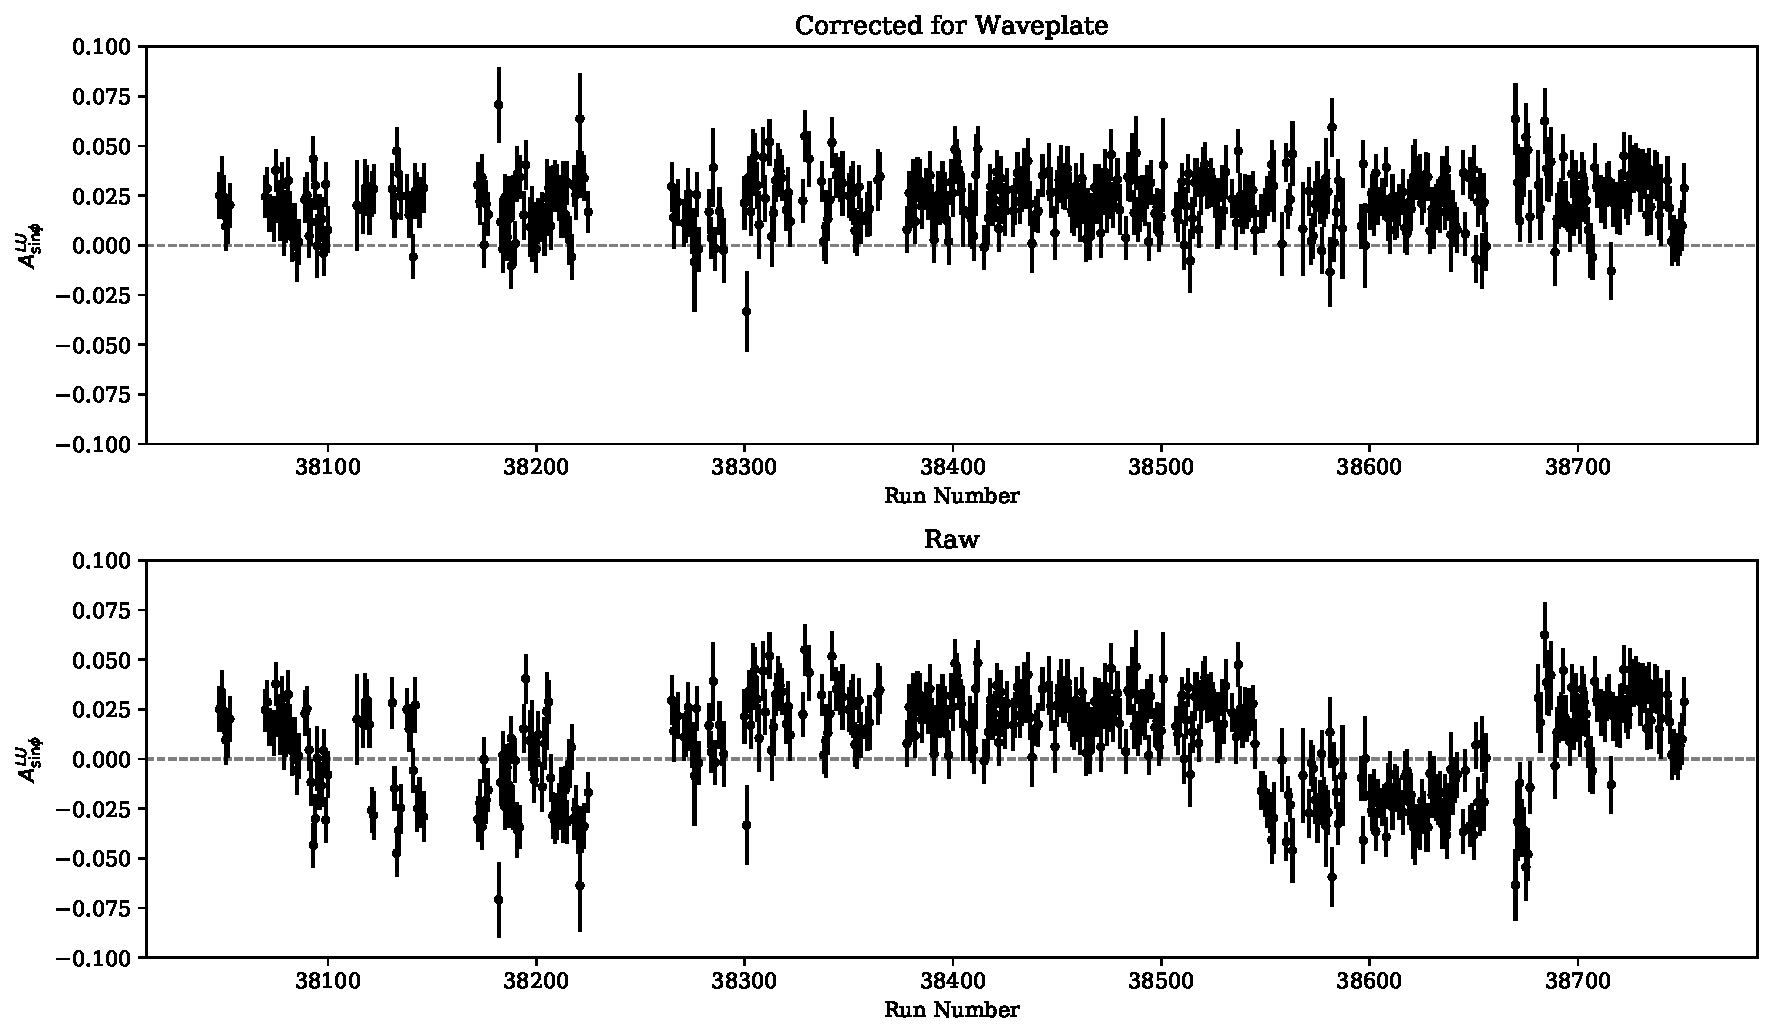
\includegraphics[width=12cm]{image/plots/basic-analysis/bsa-waveplate.pdf}
	\caption{The waveplate position is determined and corrected by plotting the BSA for $\pi^{+}$ mesons as a function of the run number.  The top panel shows the corrected results, the bottom shows the results before changing the helicity.}
\end{figure}

\section{Vertex Corrections}
The track vertex position $(v_x, v_y, v_z)$ is calculated based on the intersection of each track with the midplane (the plane which contains the beamline and bisects the sector at $\phi_{rel} = 0$).  If the beam is not centered at $(x,y)=(0,0)$, the vertex position calculation needs to be corrected by shifting the midplanes in accordance with the target offset.  The offset $(x,y)$ is identified by plotting events from the control foil placed near the target, which has a $z$ position of 20 cm. For the E1-F run period, the beam position was (0.15, -0.25) cm.  This correction is applied to the entire data set based on this position, and its successful effect is shown in figure \ref{fig:vertex_phi}.  In practice the beam position may vary more frequently than in our case, and the correction would be applied run-by-run, here it is not necessary.  \\

\begin{figure}
	\label{fig:vertex_phi}
	\begin{center}
		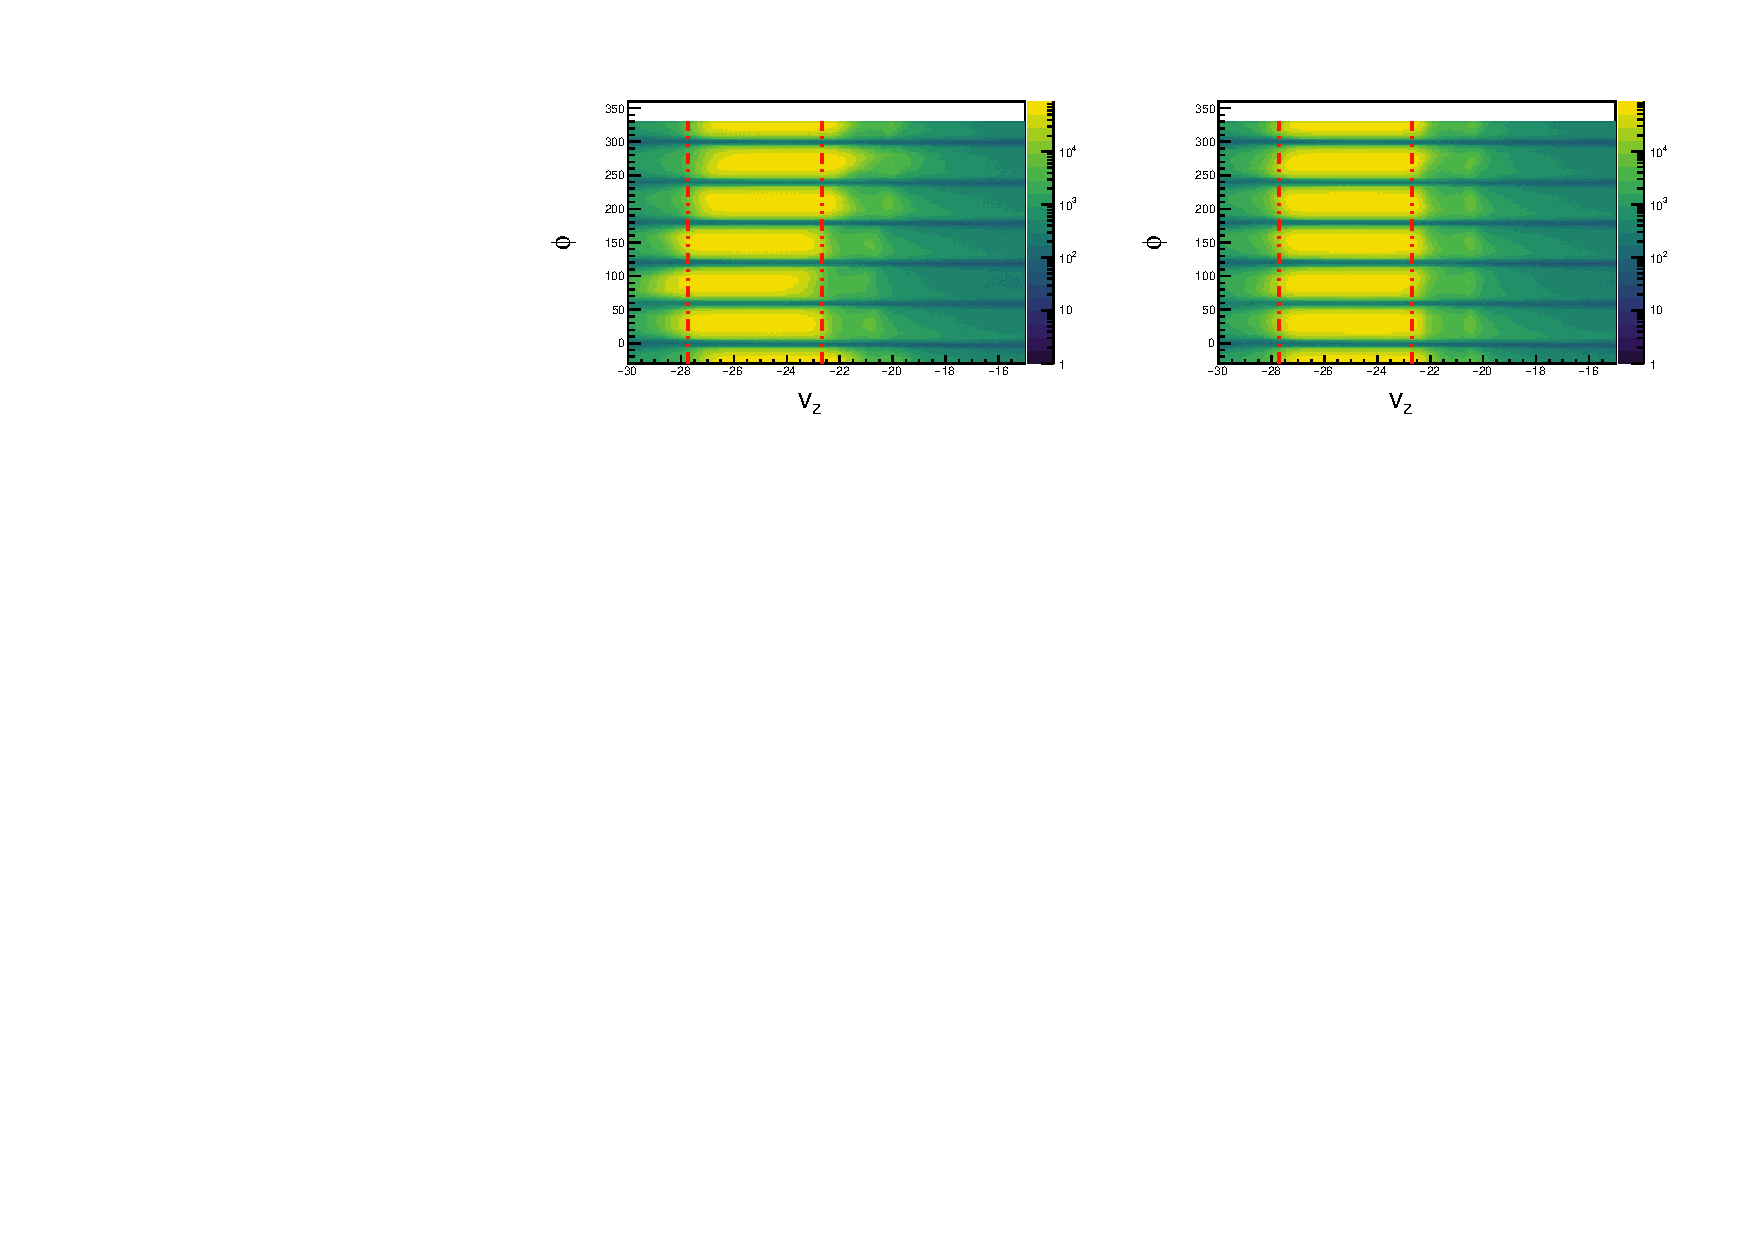
\includegraphics[width=14cm]{image/plots/basic-analysis/vertex-phi.pdf}
		\caption{The z-vertex $v_z$ position shown for different values of $\phi$ the azimuthal angle in the hall.  The left figure shows the distribution before corrections are applied, the right after.  The vertical red lines bound the region which we define as acceptable for electrons in our analysis.}
	\end{center}
\end{figure}

\section{Timing Corrections}
Timing information comes from the time-of-flight detector system.  After calibration, small offsets in timing between time of flights paddles still exist for the E1-F dataset.  These biases can be removed on a run-by-run and paddle-by-paddle basis by adding a small shift $t_{corr}$.  In order to determine this shift $t_{corr}$ for each paddle, charged pions are used.  \\

Using momentum information from the drift chambers the value of $\beta$ can be predicted and the difference $\Delta \beta$ can be determined for each pion. 

\begin{equation}
	\Delta \beta = \beta_{obs} - \beta_{pred} = \frac{d}{t_{obs}} - \sqrt{1+(m/p)^2} 
\end{equation} 

Here m (the mass of the particle detected) is assumed to be $m_{\pi}$, $t_{obs}$ refers to the measured time of flight for the particle, and d is the distance traveled in time $t_{obs}$ which comes from the fit track.  The offset $\Delta \beta$ from 0 is used to define the value of $t_{corr}$ for each paddle.  If this value is exceedingly small, no correction is applied.  For some paddles with low statistics a reasonable value for $t_{corr}$ cannot be obtained and these paddles are excluded from the analysis.  \\

\begin{figure}
	\label{fig:timing_correction}
	\centering
	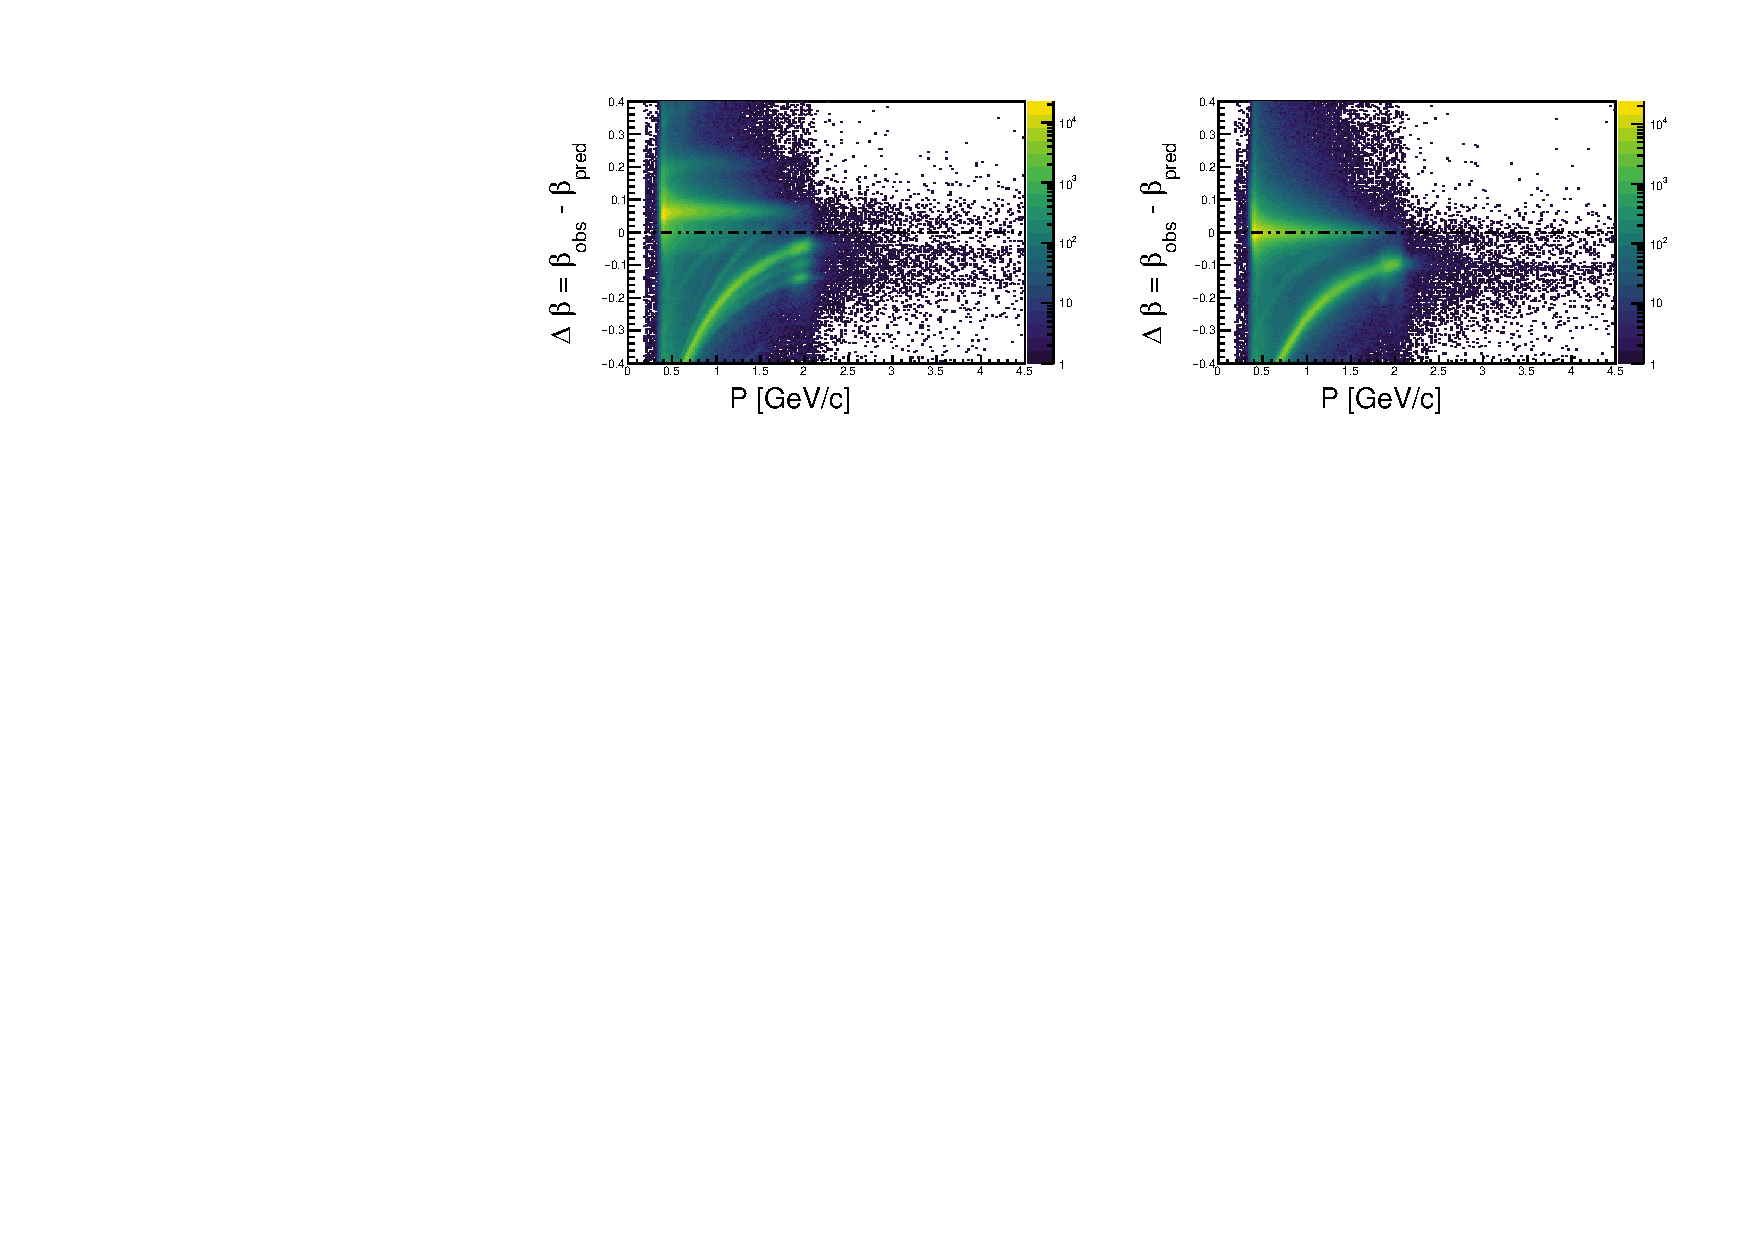
\includegraphics[width=14cm]{image/plots/basic-analysis/timing.pdf}
	\caption{Timing corrections are shown for paddle 24 of sector 1.  The left image shows the $\Delta \beta$ distribution before corrections.  On the right the same is shown after correction of the timing for this paddle.  We assume the mass of the track to be the pion, these show up as the green band.  Heavier protons are visible below the pion band.}
\end{figure}

In the method described above, the calibrated paddle is the one which is struck by the pion.  The electron paddle which was struck could also require calibration.  In practice the magnitude of the correction term $t_{corr}$ is small, and the paddle offset is (likely) randomly distributed about 0 when considering all paddles.  By including events from many different (electron) paddles, miscalibration effects from the electron side cease to be important.  This is demonstrated by the success of the technique in centering the $\Delta \beta$ distributions.  This work was first described in \cite{theses-harrison:2015}. \\

\section{Kinematic Corrections}
The magnetic field map used in reconstruction to swim particle tracks cannot perfectly match the real magnetic field of the hall.  As a result of this the reconstructed momentum of particles is often slightly off (of order 1\%).  Small misalignment in detector positions also contribute to this effect.  In order to correct for these small differences, the momentum $(p_x, p_y, p_z)$ and hence $\theta$ of charged tracks is corrected. \\

Various proceedures exist for the correction of kinematic variables of measured particles, and they all rely on energy and momentum conservation applied to standard processes (such as elastic scattering).  The procedure used to derive corrections for the E1-F dataset was developed and described by Marco Mirazita in \cite{misc-mirazita:2010}.  \\

First, elastic $(ep \rightarrow ep)$ events are selected by identifying events that contain at least one electron and one proton, then requiring that the missing mass $M_X$ of the ($ep \rightarrow epX$) system is close to 0.  The kinematics of the event are then calculated.

\begin{gather}
	k^{\mu} = (k, 0, 0, k)                         \\
	p^{\mu} = (M_{p}, 0, 0, 0)                     \\
	k'^{\mu} = (k', k'\sin\theta, 0, k'\cos\theta) \\
	p'^{\mu} = (E_{p}, -p'\sin\alpha, 0, p'\cos\alpha) 
\end{gather}

Above, the four momenta correspond to the incoming electron $k$, the outgoing electron $k'$, the stationary target proton $p$ and the scattered proton $p'$. Applying energy and momentum conservation to the equations above yields 3 equations.

\begin{gather}
	k + M_p = k' + \sqrt{M_{p}^{2} + p'^2} \\
	k'\sin\theta = p'\sin\alpha            \\
	k = k'\cos\theta + p'\cos\alpha  
\end{gather}

Using these equations, the electron angle $\theta$ and the proton angle $\alpha$ can be predicted by using the momenta $(k',p')$.  These values are compared with measured values and iteratively corrected by tuning the parameters of a phi-dependent 2nd order polynomial.

\begin{gather}
	\cos\theta = 1 - M_p \frac{k-k'}{kk'} \\
	\tan\alpha = \frac{1}{p'} \frac{k'\sin\theta}{k-k'\cos\theta}
\end{gather}

After $\theta$ corrections are applied, the momenta of the electrons are corrected by using an analogous procedure for $k'$ instead of $\theta$ and $\alpha$.  The momentum corrections are calculated as functions of $\phi$ for each sector in one degree bins of $\theta$.  Finally, the positively charged particles momenta are corrected by selecting the exclusive event $(ep \rightarrow e\pi^+N)$.  In this reaction the scattered electron and pion are detected and the neutron is selected using a missing mass cut.  Assuming the electron momentum, electron angle, and pion angle to be correct, the pion momentum correction is then calculated by iteratively improving the central position of the neutron mass peak to coincide with $M_{N}$.  Marco Mirazita shows in his note that these corrections can be satisfactorily applied to all negative and positive particles.

\easyFigure{image/plots/basic-analysis/phi-dw-uncorr.pdf}{This figure shows the deviation from $M_p$ of the $W$ spectrum peak for elastic $ep \rightarrow ep$ events (before corrections).  The six sectors of CLAS are shown here starting from 1 in the top left and ending with 6 at the bottom right.}
\easyFigure{image/plots/basic-analysis/phi-dw-corr.pdf}{This figure shows the deviation from $M_p$ of the $W$ spectrum peak for elastic $ep \rightarrow ep$ events (after $\phi$-dependent corrections).  The momentum corrections are applied as a function of $\phi$ and this plot demonstrates that the correction significantly improves the position and width of the elastic resonance in $W$ as a function of the azimuthal angle $\phi$. The six sectors of CLAS are shown here starting from 1 in the top left and ending with 6 at the bottom right.}

\begin{figure}
	\centering 
	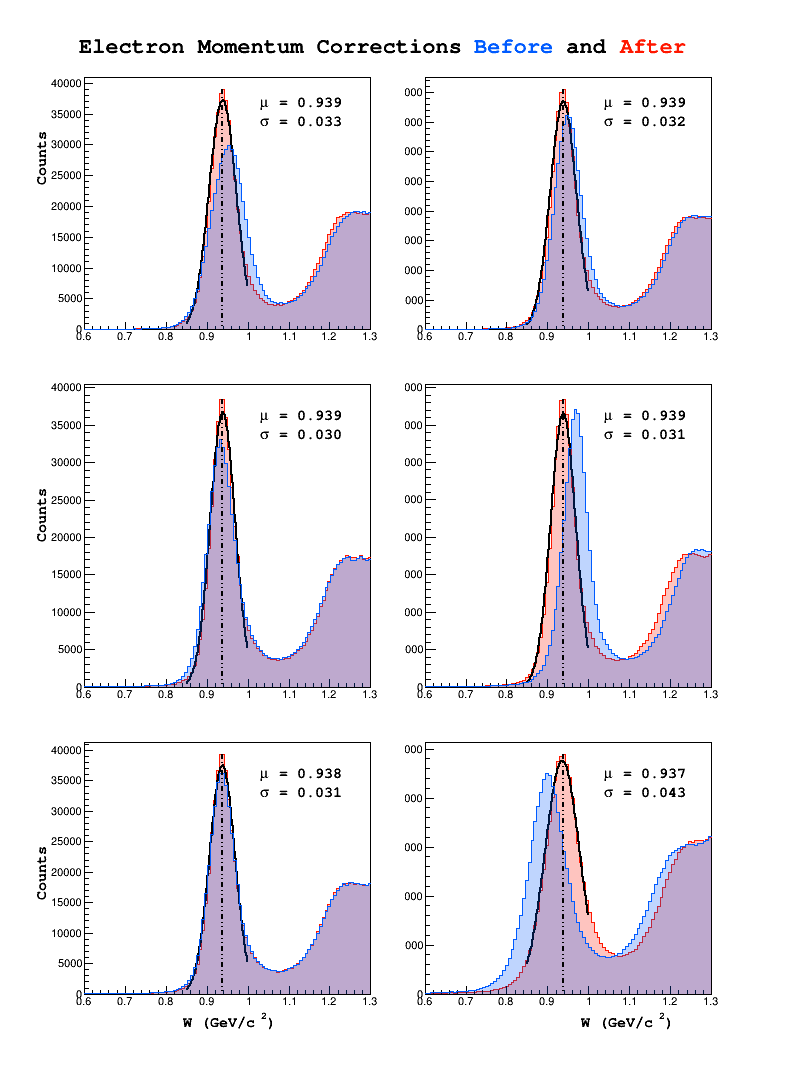
\includegraphics[width=14cm]{image/plots/basic-analysis/w-mom-corr.png}
	\caption{Elastic events shown in the spectrum of $W$ before and after momentum corrections are applied.  Each corrected sector's histogram has been fit with a Gaussian, whose mean $\mu$ and standard deviation $\sigma$ are shown on the each figure.  This figure demonstrates that they are very effective in correcting the electron kinematics.  The apparent disparity between the number of events in sectors 1-5 and sector 6 is largely an illusion due to the larger width in sector 6, in reality there is an approximate 2 percent difference in total counts between sector 6 and the other sectors average number of counts.}
\end{figure}

In this work momentum corrections are applied to the scattered electron.  We find the corrections to be very effective for all sectors, while sector 6 has a proton resonance width approximately 10 $MeV$ wider than the other sectors, this is on the order of the resolution of the detector and is likely caused by dead wires.  The central position of the proton resonance peak is corrected successfully.